	\documentclass[a4paper,12pt]{article}
%%%%%%%%%%%%%%%%%%%%%%%%%%%%%%%%%%%%%%%%%%%%%%%%%%%%%%%%%%%%%%%%%%%%%%%%%%%%%%%%%%%%%%%%%%%%%%%%%%%%%%%%%%%%%%%%%%%%%%%%%%%%%%%%%%%%%%%%%%%%%%%%%%%%%%%%%%%%%%%%%%%%%%%%%%%%%%%%%%%%%%%%%%%%%%%%%%%%%%%%%%%%%%%%%%%%%%%%%%%%%%%%%%%%%%%%%%%%%%%%%%%%%%%%%%%%
\usepackage{eurosym}
\usepackage{vmargin}
\usepackage{amsmath}
\usepackage{framed}
\usepackage{graphics}
\usepackage{epsfig}
\usepackage{subfigure}
\usepackage{enumerate}
\usepackage{fancyhdr}

\setcounter{MaxMatrixCols}{10}
%TCIDATA{OutputFilter=LATEX.DLL}
%TCIDATA{Version=5.00.0.2570}
%TCIDATA{<META NAME="SaveForMode"CONTENT="1">}
%TCIDATA{LastRevised=Wednesday, February 23, 201113:24:34}
%TCIDATA{<META NAME="GraphicsSave" CONTENT="32">}
%TCIDATA{Language=American English}

\pagestyle{fancy}
\setmarginsrb{20mm}{0mm}{20mm}{25mm}{12mm}{11mm}{0mm}{11mm}
\lhead{MS4222} \rhead{Kevin O'Brien} \chead{Binomial Distribution} %\input{tcilatex}
\begin{document}

\section*{Binomial Distribution : Probability Density Function}
A binomial experiment is one that possesses the following properties:

\begin{enumerate}
	\item The experiment consists of n repeated trials;
	
\item Each trial results in an outcome that may be classified as a success or a failure (hence the name, binomial);
	
\item The probability of a success, denoted by p, remains constant from trial to trial and repeated trials are independent.
\end{enumerate}


\noindent 
The number of successes X in n trials of a binomial experiment is called a \textbf{\textit{binomial random variable}}.


\subsection*{Binomial Probability Formula}
The probability of exactly k successes in a binomial experiment $Bin(n, p)$ is given by
\[ P(X=k) = P(k \mbox{ successes in ``n" trails }) = \;^nC_k  \times p^{k} \times (1-p)^{n-k}\]

\begin{itemize}
	\item X: Discrete random variable for the number of successes (variable name)
	\item $k$ : Number of successes (numeric value)
	\begin{itemize}
		
		\item[$\ast$]  k= 0, 1, 2, ... n
		\item[$\ast$]   $P(X=k)$ ``probability that the number of success is $k$".
	\end{itemize}
	\item $n$ : number of independent trials
	\item $p$ : probability of a success in any of the $n$ trial.
	\item $1-p$ : probability of a failure in any of the $n$ trial.
	\item ${^nC_k}$ is a combination value, found using the Choose operator.
\end{itemize}





\section*{Binomial Distribution : Expected Value and Variance}

If the random variable X has a binomial distribution with parameters $n$
and $p$, we write
\[ X \sim Bin(n,p) \]
Only these two parameters are needed to determine the probability of an event.

% Expectation and Variance
% If $X \sim B(n,p)$, then:
\begin{framed}
\begin{itemize}
	\item The expected value of $X$ is: \[\operatorname{E(X)} = n \times p \]
	\item The variance of $X$ is:
	\[\operatorname{Var(X)} = n \times p \times (1-p) = n\times p \times q \]
\end{itemize}
\end{framed}
\begin{itemize} 
	\item $p$ is the probability of success \item $q$ is the probability of failure in a binomial trial
\item $n$ is the number of independent trials \end{itemize}
\noindent \textbf{Interpretation:}
If $n=100$, and $p=0.25$, then the average number of successes will be 25.


%
%%================================================================%
%
%Suppose n=3 and p=0.5 ( like our coin flipping example for tutorial 1)
%Then E(X) = 1.5 and V(X) = 0.75.

\noindent \textbf{Remark:} Referring to the expected value and variance may be used to validate
the assumption of a binomial distribution.


\section*{Binomial Distribution : Example}

\begin{itemize} \item Diagrams of the probability mass functions of the two binomial
distributions $B(10, 0.5)$ and $B(10, 0.25)$ are shown in the bar-plots. \item Which
is which? Give a reason for your answer.
\end{itemize}
\begin{figure}[h!]
\centering
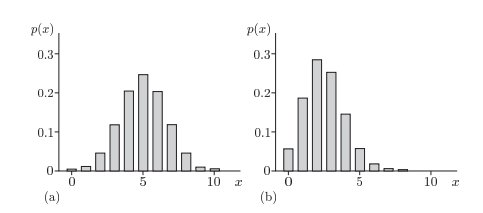
\includegraphics[width=0.7\linewidth]{images/4ABarCharts}
\label{fig:4abarcharts}
\end{figure}


\begin{itemize}
\item Figure A is $Bin(10, 0.5)$ and Figure B is $Bin(10, 0.25)$.
\item The mean of $Bin(10, 0.5)$ is 5, and the mean of B(10, 0.25) is 2.5.
\item Also the variance of a binomial distribution corresponding to $Bin(10, 0.25)$ is $1.875$ ,while for $B(10, 0.25)$ it is $2.500$.
\item A visual inspection of the two bar-charts indicates that Figure A has the higher variance.
\end{itemize}

%---------------------------------------------------------------------%

\end{document}
%--------------------------------------------------------%



